\documentclass[]{exam}
\usepackage{graphicx}
\usepackage{wrapfig}
\usepackage[utf8]{inputenc}

\title{PSYCH 511 Quiz 1}
\author{}
\date{September 14, 2018}

\pagestyle{headandfoot}
\firstpageheader{PSY 511}{}{Quiz 1}
\runningheader{PSY 511}{}{Quiz 1}
\firstpagefooter{}{Page \thepage}{}
\runningfooter{}{Page \thepage}{}

\begin{document}
\maketitle

\begin{center}
  \fbox{\fbox{\parbox{5.5in}{\centering
        Answer the questions in the spaces provided on the question sheets.
        If you run out of room for an answer, continue on the back of the page. Please take no more than 30 min to complete this quiz, and please do not use use any resources other than your own memory.}}}
\end{center}
\vspace{0.1in}
\makebox[\textwidth]{Name:\enspace\hrulefill}

\newpage

\begin{questions}

\question
\begin{parts}
\part Describe the main components of the central nervous system associated with the lateral ventricles.
\vspace{0.5in}
\part What region of the brain is associated with the cerebral aqueduct?
\vspace{0.5in}
\part What parts of the brain are associated with the 4th ventricle?
\end{parts}

\question Label the planes of section illustrated in each of the three panels in the figure below:
\vspace{0.5in}
\begin{figure}[h]
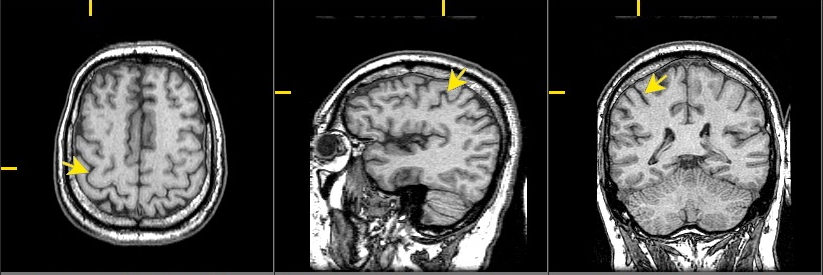
\includegraphics[width=0.80\textwidth]{511-16-quiz-1-fig-1.jpg}
\centering
\end{figure}
\vspace{0.5in}

\question The arrow in the figure above points to a major sulcus on the lateral surface of the cerebral cortex, the \fillin, which divides the \fillin from the parietal lobes.

\question Primary \fillin cortex is located on the \emph{anterior} bank of this sulcus in the \fillin lobe.

\question Primary \fillin cortex is located on the \emph{posterior} bank of this sulcus in the \fillin lobe.

\question In each of the panels in the figure, label as many of the following directional terms as you are able to use: anterior/posterior; superior/inferior; medial/lateral; dorsal/ventral. 

\question The \fillin is a forebrain structure that controls ingestion, defense, and reproductive behavior. It is also the means by which the CNS controls both the \fillin system via the pituitary gland and the \fillin nervous system.

\question The \fillin is a forebrain structure located deep within the (medial/lateral) portions of the \fillin lobe. It captures and stores behaviorally relevant information about specific places and locations.

% \question The \fillin provides a major source of input to the structure described in the previous question. Located deep in the medial \fillin lobes adjacent to the lateral ventricles, this structure is anterior to the \fillin.

\question Diffusion tensor imaging (DTI) is an example of a brain imaging technique with \fillin temporal resolution. DTI provides information about \fillin.

% \question Functional MRI (fMRI) is an example of a brain imaging technique with \fillin temporal resolution. fMRI provides information about \fillin.

\newpage

\question (2 points) Functional MRI (fMRI) is considered an \emph{indirect} measure of neuronal activity because...
\vspace{1.5in}

\question (2 points) Describe at least two ways that neurons differ from other cells in the body.
\vspace{1.5in}

\question \fillin are the type of glial cell found in the PNS; \fillin are found in the CNS.
\question Electroencephalography (EEG) measures the \fillin activity of large numbers of neurons. It is (similar to/different from) MEG in \emph{temporal} resolution.

\question (BONUS) The arrows in the figure below point to the \fillin, a structure early anatomists thought looked like a seahorse.

\vspace{0.5in}
\begin{figure}[h]
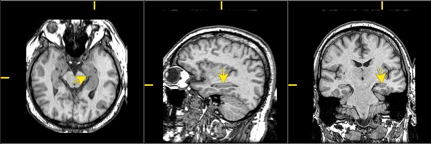
\includegraphics[width=0.80\textwidth]{quiz-1-fig-2.jpg}
\centering
\end{figure}
\vspace{0.5in}


\end{questions}
\end{document}
